\documentclass[10pt,aspectratio=169]{beamer}

\usetheme[progressbar=frametitle]{metropolis}

\newcommand{\R}{\mathbb{R}}
\renewcommand{\P}{\mathbb{P}}
\newcommand{\set}[1]{\{#1\}}

\usepackage{tikz}
\usetikzlibrary{shapes}
\usetikzlibrary{plotmarks}
\usetikzlibrary{fit}
\usetikzlibrary{overlay-beamer-styles}
\usetikzlibrary{positioning}
\usetikzlibrary{calc}
\usetikzlibrary{decorations.pathreplacing}
\usetikzlibrary{decorations.pathmorphing}
\definecolor{lightblue}{RGB}{189,216,238}

\usepackage{etoolbox}

\title{Non-Parametric Machine Learning Models for Solar Energy Forecasting}
% \subtitle{}
\date{16.07.2021}
\author{Pavel Zwerschke}
\institute{Karlsruhe Institute of Technology}
\titlegraphic{\hfill
\includegraphics[height=1.5cm]{logos/kitlogo_en_cmyk}}

\usepackage[style=authoryear, maxcitenames=2, bibencoding=inputenc]{biblatex}
\bibliography{bibliography.bib}

\begin{document}

\maketitle

\begin{frame}{Table of contents}
    \setbeamertemplate{section in toc}[sections numbered]
    \tableofcontents%[hideallsubsections]
\end{frame}

\begin{frame}{Introduction}
    \begin{itemize}
        \item Solar energy generation is characterized by fluctuations due to uncertainty of the weather
        \item Uncertainty should be quantified through a probabilistic forecast
        \begin{itemize}
            \item Probabilistic forecasts for solar energy generation are underdeveloped
            \item[\(\leadsto\)] We want to compare different machine learning based forecasting models on solar power
        \end{itemize}
    \end{itemize}
\end{frame}

\section{Model descriptions}

\begin{frame}{NNQF [\cite{Ordiano2019}]}
    \begin{center}
        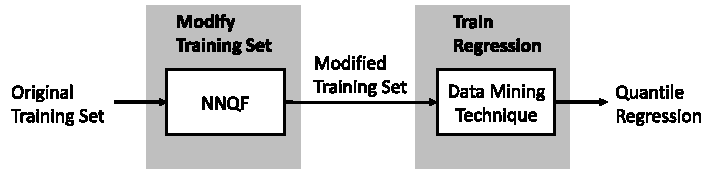
\includegraphics{plots/nnqf_approach.pdf}
    \end{center}
    \begin{itemize}
        \item Let \(x_1, \ldots, x_n \in \R^D\) be the predictors and \(y_1, \ldots, y_n\in \R\) the target values.
        \item Calculate approximate quantiles of \(y_i\):
        \begin{itemize}
            \item Find \(N\) nearest neighbors of \(x_i\): \(\set{x_{i_1}, \ldots, x_{i_N}}\)
            \item Calculate the empirical quantiles \(y_{(0.01)}, \ldots, y_{(0.99)}\) from \(\set{y_{i_1}, \ldots, y_{i_N}}\)
        \end{itemize}
    \end{itemize}
\end{frame}

\begin{frame}{NNQF [\cite{Ordiano2019}]}
    \begin{itemize}
        \item After modification of training set, a data mining technique is used for learning the map \(f(x) = (y_{(0.01)}, \ldots, y_{(0.99)})\).
        \item High correlation of adjacent data points
        \begin{itemize}
            \item[\(\leadsto\)] use lag features: don't just use \(x_i\) for prediction of \(y_i\), but also 
            \(x_{i-1}, \ldots, x_{i-H+1}\)
            \item regression model now predicts \( \P(y_i | x_i, \ldots, x_{i-H+1}) \)
        \end{itemize}
    \end{itemize}
\end{frame}

\begin{frame}{Advantages of NNQF [\cite{Ordiano2019}]}
    \begin{itemize}
        \item the regression technique is not specified, any technique can be used
        \begin{itemize}
            \item in the classical quantile regression techniques and QRF, the algorithm needs to be specified
        \end{itemize}
        \item nearest neighbor calculation only needs to be done once
        \begin{itemize}
            \item nearest neighbor quantile regression calculates the nearest neighbors for each prediction
        \end{itemize}
        \item the original dataset does not need to be saved
    \end{itemize}
\end{frame}

\begin{frame}{QRF [\cite{Meinshausen2006}]}
    \begin{itemize}
        \item Use bagging to produce \(k\) trees from training set \(x_1, \ldots, x_n \in \R^D\) and \(y_1, \ldots, y_n \in \R\)
        \item For \(x\in \R^D\), we want to predict the distribution \(\P(Y | X=x)\)
        \begin{itemize}
            \item Calculate \(\hat{y}_1, \ldots, \hat{y}_k\) from the trees 
            \item Calculate the empirical quantiles \(\hat{y}_{(q)}\) of \(\set{\hat{y}_1, \ldots, \hat{y}_k}\) for any \(q \in (0,1)\)
        \end{itemize}
    \end{itemize}
\end{frame}

\begin{frame}[fragile]{DeepAR -- Training [\cite{Salinas2017}]}
    \begin{center}
        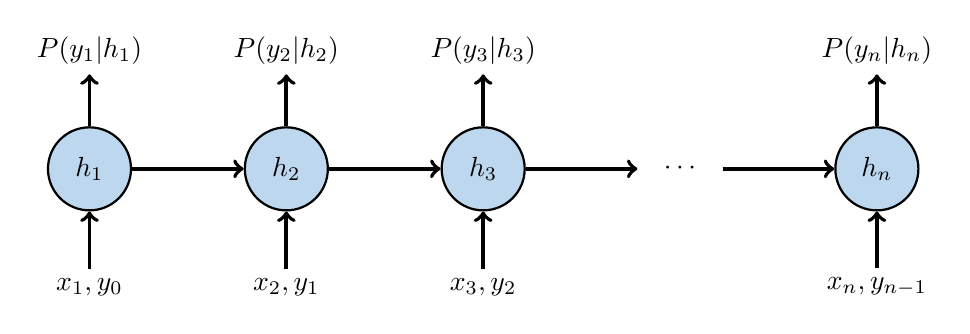
\begin{tikzpicture}[yscale=-1,node distance=-\pgflinewidth]
    \tikzset{ReceptorNode/.style={circle, draw=black, fill=lightblue, thick, inner sep=2pt, minimum size=30pt}}
    \tikzset{Placeholder/.style={circle, thick, inner sep=2pt, minimum size=30pt}}
    \tikzset{Connection/.style={->, line width=0.5mm}}
    \newcommand{\mynode}[3]{
        \node[ReceptorNode] (circ-#2) at (#1, 0) {\(\boldsymbol{h}_{#2}\)};
        \node (x-#2) at (#1, 1.5) {\(x_{#2}, y_{#3}\)};
        \node (y-#2) at (#1, -1.5) {\(\P(y_{#2}|\boldsymbol{h}_{#2})\)};

        \draw[Connection] (circ-#2) -- (y-#2);
        \draw[Connection] (x-#2)    -- (circ-#2);
    }
    \newcommand{\placeholder}[2]{
        \node[Placeholder] (circ-#2) at (#1, 0) {\(\cdots\)};
        \node (x-#2) at (#1, 1.5) {};
        \node (y-#2) at (#1, -1.5) {\phantom{\(\P(y_{#2}|\boldsymbol{h}_{#2})\)}};
    }
    \newcommand{\connect}[2]{
        \draw[Connection] (circ-#1) -- (circ-#2);
    }

    % Create nodes
    \mynode{1 * 2.5}{1}{0}
    \onslide<2->{
        \mynode{2 * 2.5}{2}{1}
        \connect{1}{2}    
    }
    \onslide<2->{
        \mynode{3 * 2.5}{3}{2}
        \connect{2}{3}    
    }
    \onslide<3->{
        \placeholder{4 * 2.5}{4}
        \connect{3}{4}
    }
    % Last node is called "n"
    \onslide<4->{
        \mynode{5*2.5}{n}{n-1}
        \connect{4}{n}
    }
\end{tikzpicture}
    \end{center}
    \begin{itemize}
        \item Autoregressive Recurrent Neural Network with probabilistic output
        \item \(x_t\) and \(z_{t-1}\) form with \(\boldsymbol{h}_{t-1}\) the new network output \(\boldsymbol{h}_t\)
        which is used to compute the likelihood \(\P(z_t | \boldsymbol{h}_t)\)
    \end{itemize}
\end{frame}

\begin{frame}[fragile]{DeepAR -- Predicting [\cite{Salinas2017}]}
    \begin{center}
        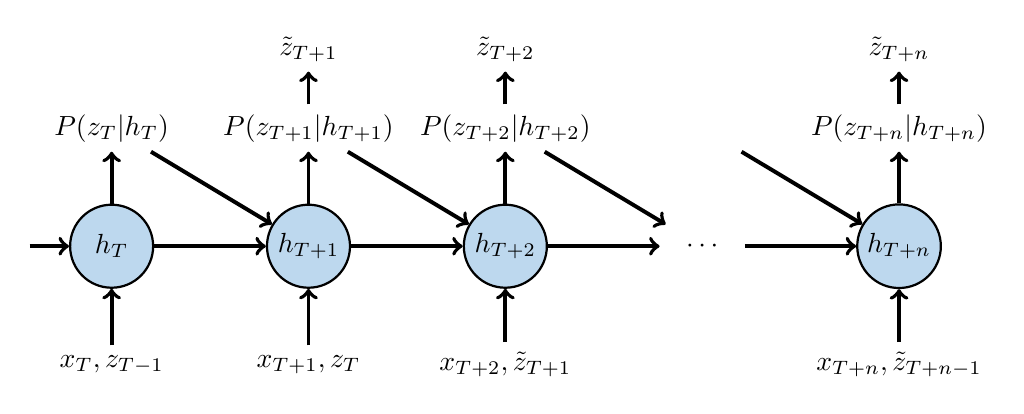
\begin{tikzpicture}[yscale=-1,node distance=-\pgflinewidth]
    \tikzset{ReceptorNode/.style={circle, draw=black, fill=lightblue, thick, inner sep=2pt, minimum size=30pt}}
    \tikzset{Placeholder/.style={circle, thick, inner sep=2pt, minimum size=30pt}}
    \tikzset{Connection/.style={->, line width=0.5mm}}
    \newcommand{\mynode}[3]{
        \node[ReceptorNode] (circ-#2) at (#1, 0) {\(\boldsymbol{h}_{#2}\)};
        \node (x-#2) at (#1, 1.5) {\(x_{#2}, z_{#3}\)};
        \node (y-#2) at (#1, -1.5) {\(\P(z_{#2}|\boldsymbol{h}_{#2})\)};

        \draw[Connection] (circ-#2) -- (y-#2);
        \draw[Connection] (x-#2)    -- (circ-#2);
    }
    \newcommand{\mynodewithresult}[3]{
        \node[ReceptorNode] (circ-#2) at (#1, 0) {\(\boldsymbol{h}_{#2}\)};
        \node (x-#2) at (#1, 1.5) {\(x_{#2}, z_{#3}\)};
        \node (y-#2) at (#1, -1.5) {\(\P(z_{#2}|\boldsymbol{h}_{#2})\)};
        \node (z-#2) at (#1, -2.5) {\(\tilde{z}_{#2}\)};

        \draw[Connection] (circ-#2) -- (y-#2);
        \draw[Connection] (x-#2)    -- (circ-#2);
        \draw[Connection] (y-#2)    -- (z-#2);
    }
    \newcommand{\mynodewithresultinputsampled}[3]{
        \node[ReceptorNode] (circ-#2) at (#1, 0) {\(\boldsymbol{h}_{#2}\)};
        \node (x-#2) at (#1, 1.5) {\(x_{#2}, \tilde{z}_{#3}\)};
        \node (y-#2) at (#1, -1.5) {\(\P(z_{#2}|\boldsymbol{h}_{#2})\)};
        \node (z-#2) at (#1, -2.5) {\(\tilde{z}_{#2}\)};

        \draw[Connection] (circ-#2) -- (y-#2);
        \draw[Connection] (x-#2)    -- (circ-#2);
        \draw[Connection] (y-#2)    -- (z-#2);
    }
    \newcommand{\placeholder}[2]{
        \node[Placeholder] (circ-#2) at (#1, 0) {\(\cdots\)};
        \node (x-#2) at (#1, 1.5) {};
        \node[opacity=0] (y-#2) at (#1, -1.5) {\(\P(z_{#2}|h_{#2})\)};
    }
    \newcommand{\connect}[2]{
        \draw[Connection] (y-#1)    -- (circ-#2);
        \draw[Connection] (circ-#1) -- (circ-#2);
    }

    % Create nodes
    \mynode{1 * 2.5}{T}{T-1}
    \draw[Connection] ([xshift=-0.5cm]circ-T.west) -- (circ-T);
    \onslide<2->{
        \mynodewithresult{2 * 2.5}{T+1}{T}
        \connect{T}{T+1}
    }
    \onslide<3->{
        \mynodewithresultinputsampled{3 * 2.5}{T+2}{T+1}
        \connect{T+1}{T+2}
    }
    \onslide<4->{
        \placeholder{4 * 2.5}{T+3}
        \connect{T+2}{T+3}
    }
    % Last node is called "T+n"
    \onslide<5->{
        \mynodewithresultinputsampled{5*2.5}{T+n}{T+n-1}
        \connect{T+3}{T+n}
    }
\end{tikzpicture}
    \end{center}
    \begin{itemize}
        \onslide<2->{\item Generate \(\tilde{z}_t \sim \P(\cdot | \boldsymbol{h}_t)\) and use it in the next step as input}
    \end{itemize}
\end{frame}

\begin{frame}{SQF-RNN [\cite{Gasthaus2019}]}
    \begin{columns}
    \begin{column}{0.6\textwidth}
    \begin{itemize}
        \item Main difference to DeepAR is output distribution
        \begin{itemize}
            \item Given by monotonously increasing linear splines: 
            \[ s(x; \gamma, b, d) = \gamma + \sum_{l=0}^L b_l (x - d_l)_+ \]
            \item Arbitrary distribution can be fit \(\leadsto\) no assumption on distribution
        \end{itemize}
    \end{itemize}
    \end{column}

    \begin{column}{0.35\textwidth}
        \begin{tikzpicture}[scale=0.6]
    \pgfplotsset{every axis/.style={mlineplot}}
    \begin{axis}[xmin=-0.05, xmax=1.05, ymin=-0.1, ymax=2.1]
        \addplot[domain = 0:1] {tanh(4*x-2)-tanh(-2)};
        \addplot[domain = 0:0.3] {x};
        \addplot[domain = 0.3:0.7] {0.3 + 3.3 * (x - 0.3)};
        \addplot[domain = 0.7:1] {1.62 + 1.02 * (x - 0.7)};
    \end{axis}
\end{tikzpicture}
    \end{column}
    \end{columns}
\end{frame}

\begin{frame}{Summary}
    \begin{itemize}
        \item NNQF
        \begin{itemize}
            \item Preprocessing with nearest neighbor filters \(\leadsto\) regression for preprocessed data
        \end{itemize}
        \item QRF
        \begin{itemize}
            \item Random Forests \(\leadsto\) take empirical quantiles of result
        \end{itemize}
        \item SQF-RNN
        \begin{itemize}
            \item Deep neural network with autoregressive input
            \item Target distribution modeled by spline quantile functions
        \end{itemize}
    \end{itemize}
\end{frame}

\begin{frame}{Plots}
    \begin{columns}
        \begin{column}{0.33\textwidth}
            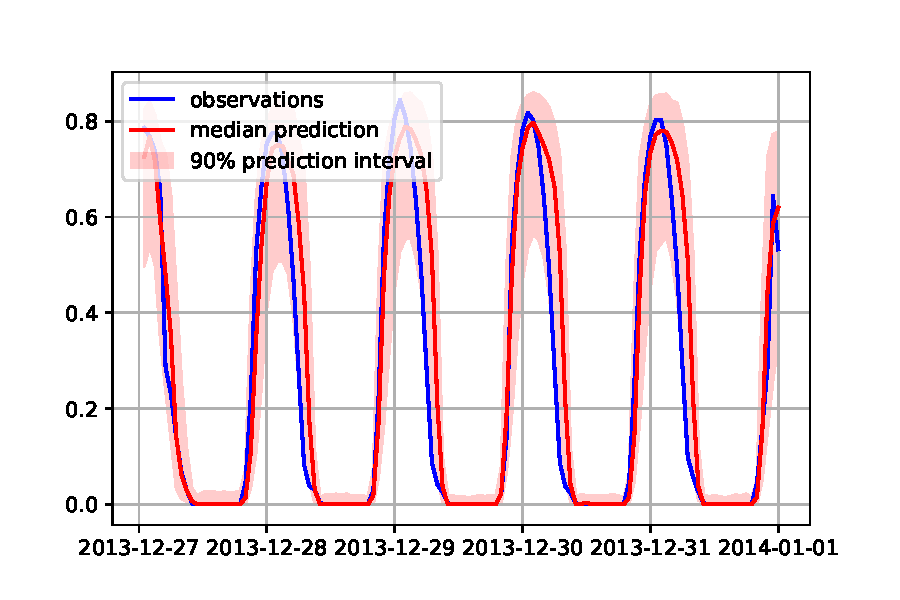
\includegraphics[width=\textwidth]{plots/nnqf_plot_9.pdf}
            \begin{center}
                NNQF
            \end{center}
        \end{column}
        \begin{column}{0.33\textwidth}
            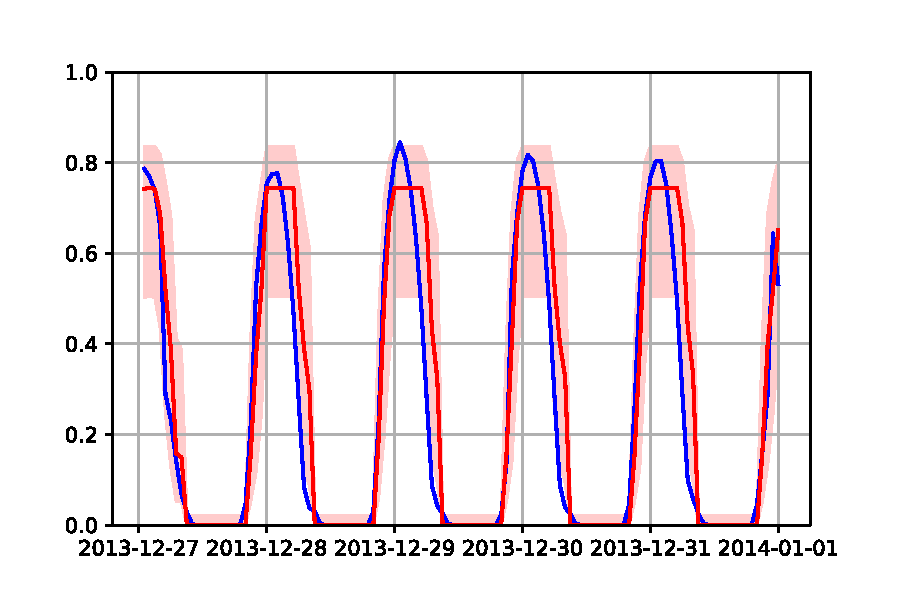
\includegraphics[width=\textwidth]{plots/qrf_plot_9.pdf}
            \begin{center}
                QRF
            \end{center}
        \end{column}
        \begin{column}{0.33\textwidth}
            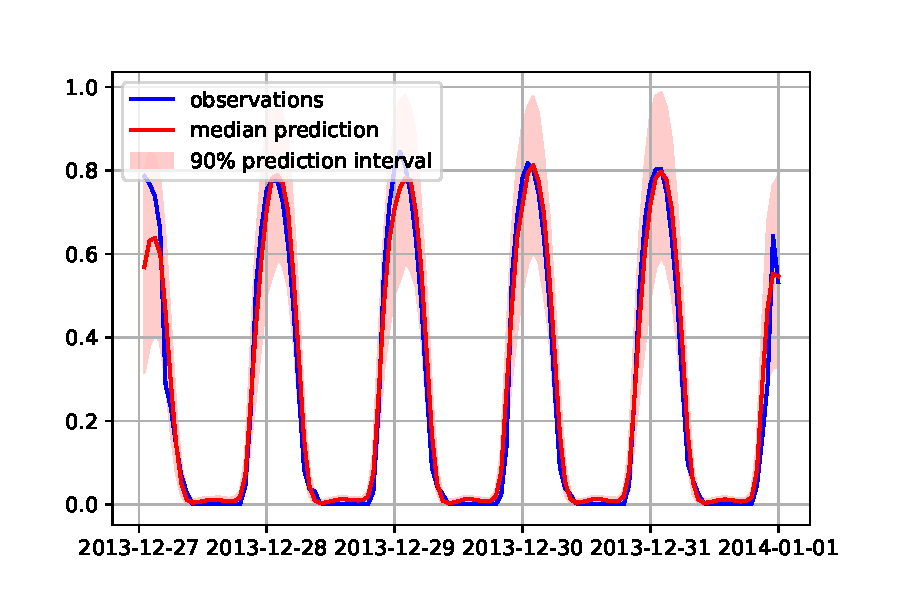
\includegraphics[width=\textwidth]{plots/sqf_rnn_plot_9.pdf}
            \begin{center}
                SQF-RNN
            \end{center}
        \end{column}
    \end{columns}
\end{frame}

\section{Comparison}

\begin{frame}{Feature importance}
    \begin{center}
        \section{Feature importance}
\label{sec:feature-importance}

One way to determine the importance of a feature for a model is called 
permutation feature importance. Here, the model is trained like usual but for the prediction 
step, we don't use the normal test data, but a modified dataset where one feature is 
shuffled. Like that, the model cannot use the information of this feature properly 
and will most likely perform worse. The performance on the shuffled dataset is 
then divided by the performance on the regular test set. A value close to \(1\) 
indicates that the feature is not that important because the model doesn't perform 
much worse than before. The higher the quotient, the more important the feature is for the model.
Since our time series heavily depends of the time of day, it makes sense 
not to shuffle the whole feature but only the equivalence classes of each hour, 
i.e. the values at \(1\) AM are shuffled, the values at \(2\) AM are shuffled, etc.

Figure \ref{fig:feature-importance} 
shows the results of the permutation feature importance calculation.

\begin{figure}[h!]
    \section{Feature importance}
\label{sec:feature-importance}

One way to determine the importance of a feature for a model is called 
permutation feature importance. Here, the model is trained like usual but for the prediction 
step, we don't use the normal test data, but a modified dataset where one feature is 
shuffled. Like that, the model cannot use the information of this feature properly 
and will most likely perform worse. The performance on the shuffled dataset is 
then divided by the performance on the regular test set. A value close to \(1\) 
indicates that the feature is not that important because the model doesn't perform 
much worse than before. The higher the quotient, the more important the feature is for the model.
Since our time series heavily depends of the time of day, it makes sense 
not to shuffle the whole feature but only the equivalence classes of each hour, 
i.e. the values at \(1\) AM are shuffled, the values at \(2\) AM are shuffled, etc.

Figure \ref{fig:feature-importance} 
shows the results of the permutation feature importance calculation.

\begin{figure}[h!]
    \section{Feature importance}
\label{sec:feature-importance}

One way to determine the importance of a feature for a model is called 
permutation feature importance. Here, the model is trained like usual but for the prediction 
step, we don't use the normal test data, but a modified dataset where one feature is 
shuffled. Like that, the model cannot use the information of this feature properly 
and will most likely perform worse. The performance on the shuffled dataset is 
then divided by the performance on the regular test set. A value close to \(1\) 
indicates that the feature is not that important because the model doesn't perform 
much worse than before. The higher the quotient, the more important the feature is for the model.
Since our time series heavily depends of the time of day, it makes sense 
not to shuffle the whole feature but only the equivalence classes of each hour, 
i.e. the values at \(1\) AM are shuffled, the values at \(2\) AM are shuffled, etc.

Figure \ref{fig:feature-importance} 
shows the results of the permutation feature importance calculation.

\begin{figure}[h!]
    \input{plots/feature_importance}
    \caption[Feature importance]{Feature importance. 
    The table shows the permutation feature importance quotients. 
    The permutation feature importance quotient is 
    the performance of the model with shuffled feature 
    divided by the performance of the model without shuffled features. 
    A higher value indicates a more important feature.}
    \label{fig:feature-importance}
\end{figure}
    \caption[Feature importance]{Feature importance. 
    The table shows the permutation feature importance quotients. 
    The permutation feature importance quotient is 
    the performance of the model with shuffled feature 
    divided by the performance of the model without shuffled features. 
    A higher value indicates a more important feature.}
    \label{fig:feature-importance}
\end{figure}
    \caption[Feature importance]{Feature importance. 
    The table shows the permutation feature importance quotients. 
    The permutation feature importance quotient is 
    the performance of the model with shuffled feature 
    divided by the performance of the model without shuffled features. 
    A higher value indicates a more important feature.}
    \label{fig:feature-importance}
\end{figure}
    \end{center}
\end{frame}

\begin{frame}[fragile]{Pinball loss}
    \begin{columns}
    \begin{column}{0.5\textwidth}
        \begin{flushright}
            \section{Pinball Loss}
\label{sec:elaboration-pinball-loss}

As stated in section \ref{sec:pinball-loss-explanation}, the pinball loss is 
used to determine the performance of the different models. 
It is calculated by taking the average over all pinball losses for each time 
point and zone in the dataset. 

Table \ref{table:pinball-loss} and Figure \ref{fig:pinball-loss} show the 
losses of the models for task 4 to task 15 (July 2013 to June 2014). 
We can see that the QRF and NNQF model perform similarly and that the 
SQF-RNN model performs better than the other two during the months from October to Febuary.
Another thing to note is that the DeepAR model always performs worse than the SQF-RNN model.

\begin{table}[ht]%
    \footnotesize
    \hspace*{25pt} % make kind of centering
    \begin{minipage}{\textwidth}
    \renewcommand{\b}[1]{\textbf{#1}}
    \rowcolors{2}{white}{gray!25}
    \begin{tabular}{c|cccccc}
        \toprule \noalign{\smallskip}
        Task & \(4\) & \(5\) & \(6\) & \(7\) & \(8\) & \(9\) \\
        \midrule
        QRF     & \(\b{0.01462}\) & \(\b{0.02022}\) & \(\b{0.01884}\) & \(0.02250\)     & \(0.02258\)     & \(0.02212\)     \\
        NNQF    & \(0.01559\)     & \(0.02091\)     & \(0.01896\)     & \(0.02267\)     & \(0.02330\)     & \(0.02334\)     \\
        SQF-RNN & \(0.02581\)     & \(0.03041\)     & \(0.02451\)     & \(\b{0.01895}\) & \(\b{0.01707}\) & \(\b{0.01833}\) \\
        DeepAR  & \(0.02634\)     & \(0.03649\)     & \(0.02744\)     & \(0.01958\)     & \(0.02579\)     & \(0.02290\)     \\
        \bottomrule
    \end{tabular}
    \vspace*{1em} \\
    \rowcolors{2}{white}{gray!25}
    \begin{tabular}{c|cccccc|c}
        \toprule \noalign{\smallskip}
        Task & \(10\) & \(11\) & \(12\) & \(13\) & \(14\) & \(15\) & Mean \\
        \midrule
        QRF     & \(0.02232\)     & \(\b{0.02012}\) & \(\b{0.01824}\) & \(\b{0.01561}\) & \(\b{0.01355}\) & \(\b{0.01402}\) & \(\b{0.01873}\) \\
        NNQF    & \(0.02333\)     & \(0.02038\)     & \(0.01912\)     & \(0.01673\)     & \(0.01363\)     & \(0.01480\)     & \(0.01940\)     \\
        SQF-RNN & \(\b{0.02002}\) & \(0.02104\)     & \(0.02204\)     & \(0.01684\)     & \(0.01338\)     & \(0.01648\)     & \(0.02041\)     \\
        DeepAR  & \(0.02320\)     & \(0.02612\)     & \(0.02424\)     & \(0.02282\)     & \(0.01865\)     & \(0.01889\)     & \(0.02437\)     \\
        \bottomrule
    \end{tabular}
    \end{minipage}

    \caption[Pinball loss]{Pinball loss. 
    Each task is one month in the training period. 
    Task 4 represents July 2013, Task 5 August 2013, etc. up until June 2014.
    The pinball loss is calculated by averaging 
    over all pinball losses for each time point and zone.}
    \label{table:pinball-loss}
\end{table}

\begin{figure}[ht]
    \centering
    \section{Pinball Loss}
\label{sec:elaboration-pinball-loss}

As stated in section \ref{sec:pinball-loss-explanation}, the pinball loss is 
used to determine the performance of the different models. 
It is calculated by taking the average over all pinball losses for each time 
point and zone in the dataset. 

Table \ref{table:pinball-loss} and Figure \ref{fig:pinball-loss} show the 
losses of the models for task 4 to task 15 (July 2013 to June 2014). 
We can see that the QRF and NNQF model perform similarly and that the 
SQF-RNN model performs better than the other two during the months from October to Febuary.
Another thing to note is that the DeepAR model always performs worse than the SQF-RNN model.

\begin{table}[ht]%
    \footnotesize
    \hspace*{25pt} % make kind of centering
    \begin{minipage}{\textwidth}
    \renewcommand{\b}[1]{\textbf{#1}}
    \rowcolors{2}{white}{gray!25}
    \begin{tabular}{c|cccccc}
        \toprule \noalign{\smallskip}
        Task & \(4\) & \(5\) & \(6\) & \(7\) & \(8\) & \(9\) \\
        \midrule
        QRF     & \(\b{0.01462}\) & \(\b{0.02022}\) & \(\b{0.01884}\) & \(0.02250\)     & \(0.02258\)     & \(0.02212\)     \\
        NNQF    & \(0.01559\)     & \(0.02091\)     & \(0.01896\)     & \(0.02267\)     & \(0.02330\)     & \(0.02334\)     \\
        SQF-RNN & \(0.02581\)     & \(0.03041\)     & \(0.02451\)     & \(\b{0.01895}\) & \(\b{0.01707}\) & \(\b{0.01833}\) \\
        DeepAR  & \(0.02634\)     & \(0.03649\)     & \(0.02744\)     & \(0.01958\)     & \(0.02579\)     & \(0.02290\)     \\
        \bottomrule
    \end{tabular}
    \vspace*{1em} \\
    \rowcolors{2}{white}{gray!25}
    \begin{tabular}{c|cccccc|c}
        \toprule \noalign{\smallskip}
        Task & \(10\) & \(11\) & \(12\) & \(13\) & \(14\) & \(15\) & Mean \\
        \midrule
        QRF     & \(0.02232\)     & \(\b{0.02012}\) & \(\b{0.01824}\) & \(\b{0.01561}\) & \(\b{0.01355}\) & \(\b{0.01402}\) & \(\b{0.01873}\) \\
        NNQF    & \(0.02333\)     & \(0.02038\)     & \(0.01912\)     & \(0.01673\)     & \(0.01363\)     & \(0.01480\)     & \(0.01940\)     \\
        SQF-RNN & \(\b{0.02002}\) & \(0.02104\)     & \(0.02204\)     & \(0.01684\)     & \(0.01338\)     & \(0.01648\)     & \(0.02041\)     \\
        DeepAR  & \(0.02320\)     & \(0.02612\)     & \(0.02424\)     & \(0.02282\)     & \(0.01865\)     & \(0.01889\)     & \(0.02437\)     \\
        \bottomrule
    \end{tabular}
    \end{minipage}

    \caption[Pinball loss]{Pinball loss. 
    Each task is one month in the training period. 
    Task 4 represents July 2013, Task 5 August 2013, etc. up until June 2014.
    The pinball loss is calculated by averaging 
    over all pinball losses for each time point and zone.}
    \label{table:pinball-loss}
\end{table}

\begin{figure}[ht]
    \centering
    \section{Pinball Loss}
\label{sec:elaboration-pinball-loss}

As stated in section \ref{sec:pinball-loss-explanation}, the pinball loss is 
used to determine the performance of the different models. 
It is calculated by taking the average over all pinball losses for each time 
point and zone in the dataset. 

Table \ref{table:pinball-loss} and Figure \ref{fig:pinball-loss} show the 
losses of the models for task 4 to task 15 (July 2013 to June 2014). 
We can see that the QRF and NNQF model perform similarly and that the 
SQF-RNN model performs better than the other two during the months from October to Febuary.
Another thing to note is that the DeepAR model always performs worse than the SQF-RNN model.

\begin{table}[ht]%
    \footnotesize
    \hspace*{25pt} % make kind of centering
    \begin{minipage}{\textwidth}
    \renewcommand{\b}[1]{\textbf{#1}}
    \rowcolors{2}{white}{gray!25}
    \begin{tabular}{c|cccccc}
        \toprule \noalign{\smallskip}
        Task & \(4\) & \(5\) & \(6\) & \(7\) & \(8\) & \(9\) \\
        \midrule
        QRF     & \(\b{0.01462}\) & \(\b{0.02022}\) & \(\b{0.01884}\) & \(0.02250\)     & \(0.02258\)     & \(0.02212\)     \\
        NNQF    & \(0.01559\)     & \(0.02091\)     & \(0.01896\)     & \(0.02267\)     & \(0.02330\)     & \(0.02334\)     \\
        SQF-RNN & \(0.02581\)     & \(0.03041\)     & \(0.02451\)     & \(\b{0.01895}\) & \(\b{0.01707}\) & \(\b{0.01833}\) \\
        DeepAR  & \(0.02634\)     & \(0.03649\)     & \(0.02744\)     & \(0.01958\)     & \(0.02579\)     & \(0.02290\)     \\
        \bottomrule
    \end{tabular}
    \vspace*{1em} \\
    \rowcolors{2}{white}{gray!25}
    \begin{tabular}{c|cccccc|c}
        \toprule \noalign{\smallskip}
        Task & \(10\) & \(11\) & \(12\) & \(13\) & \(14\) & \(15\) & Mean \\
        \midrule
        QRF     & \(0.02232\)     & \(\b{0.02012}\) & \(\b{0.01824}\) & \(\b{0.01561}\) & \(\b{0.01355}\) & \(\b{0.01402}\) & \(\b{0.01873}\) \\
        NNQF    & \(0.02333\)     & \(0.02038\)     & \(0.01912\)     & \(0.01673\)     & \(0.01363\)     & \(0.01480\)     & \(0.01940\)     \\
        SQF-RNN & \(\b{0.02002}\) & \(0.02104\)     & \(0.02204\)     & \(0.01684\)     & \(0.01338\)     & \(0.01648\)     & \(0.02041\)     \\
        DeepAR  & \(0.02320\)     & \(0.02612\)     & \(0.02424\)     & \(0.02282\)     & \(0.01865\)     & \(0.01889\)     & \(0.02437\)     \\
        \bottomrule
    \end{tabular}
    \end{minipage}

    \caption[Pinball loss]{Pinball loss. 
    Each task is one month in the training period. 
    Task 4 represents July 2013, Task 5 August 2013, etc. up until June 2014.
    The pinball loss is calculated by averaging 
    over all pinball losses for each time point and zone.}
    \label{table:pinball-loss}
\end{table}

\begin{figure}[ht]
    \centering
    \input{plots/pinball_loss}
    \caption[Pinball loss]{Pinball loss. 
    This graph plots the losses of the models for each month of the dataset competition.}
    \label{fig:pinball-loss}
\end{figure}

As described in section \ref{sec:implementation-nnqf}, 
we only use one neural network with more hidden nodes instead of 
separate neural networks for each node. 
The pinball loss for training the model with \(99\) different neural networks 
is \(0.01998\), so the version with one neural network performs approximately the 
same while being noticably faster. 
Another modification to the original algorithm proposed by \Textcite{Ordiano2019} 
is sorting the predicted quantiles instead of taking the maximum as described in 
section \ref{sec:implementation-nnqf}. The avergae pinball loss over all tasks for the second is 
\(0.02742\), so sorting the quantiles instead of taking the maximum of the previous quantile 
results in a noticable performance improvement.
    \caption[Pinball loss]{Pinball loss. 
    This graph plots the losses of the models for each month of the dataset competition.}
    \label{fig:pinball-loss}
\end{figure}

As described in section \ref{sec:implementation-nnqf}, 
we only use one neural network with more hidden nodes instead of 
separate neural networks for each node. 
The pinball loss for training the model with \(99\) different neural networks 
is \(0.01998\), so the version with one neural network performs approximately the 
same while being noticably faster. 
Another modification to the original algorithm proposed by \Textcite{Ordiano2019} 
is sorting the predicted quantiles instead of taking the maximum as described in 
section \ref{sec:implementation-nnqf}. The avergae pinball loss over all tasks for the second is 
\(0.02742\), so sorting the quantiles instead of taking the maximum of the previous quantile 
results in a noticable performance improvement.
    \caption[Pinball loss]{Pinball loss. 
    This graph plots the losses of the models for each month of the dataset competition.}
    \label{fig:pinball-loss}
\end{figure}

As described in section \ref{sec:implementation-nnqf}, 
we only use one neural network with more hidden nodes instead of 
separate neural networks for each node. 
The pinball loss for training the model with \(99\) different neural networks 
is \(0.01998\), so the version with one neural network performs approximately the 
same while being noticably faster. 
Another modification to the original algorithm proposed by \Textcite{Ordiano2019} 
is sorting the predicted quantiles instead of taking the maximum as described in 
section \ref{sec:implementation-nnqf}. The avergae pinball loss over all tasks for the second is 
\(0.02742\), so sorting the quantiles instead of taking the maximum of the previous quantile 
results in a noticable performance improvement.
        \end{flushright}
    \end{column}
    \begin{column}{0.5\textwidth}
        Mean losses:
        \begin{description}
            \item[\textcolor{TolDarkBlue}{NNQF}] \(0.01940\), place 16/24
            \item[\textcolor{TolLightBrown}{QRF}] \(0.02015\), place 17/24
            \item[\textcolor{TolLightGreen}{SQF-RNN}] \(0.02041\), place 18/24
            \item[\textcolor{TolDarkBrown}{DeepAR}] \(0.02437\), place 20/24
        \end{description}
    \end{column}
    \end{columns}
    
    \begin{itemize}
        \item NNQF and QRF perform very similar
        \item In the summer months (southern hemisphere!), SQF-RNN performs noticably better than NNQF and QRF models
        \begin{itemize}
            \item[\(\leadsto\)] NNQF and QRF only focus on solar radiation, not on total cloud cover
        \end{itemize}
    \end{itemize}
\end{frame}

\begin{frame}[fragile]{Energy score}
    \begin{columns}
    \begin{column}{0.5\textwidth}
    \begin{flushright}
        \begin{tikzpicture}[scale=0.6]
    \pgfplotsset{every axis/.style={mlineplot}}
    \begin{axis}[title=Energy score, 
                 xlabel=Month, 
                 ylabel=loss, 
                 xtick={4,6,8,10,12,14}, 
                 xticklabels={Jul, Sep, Nov, Jan, Mar, May}]
        % NNQF
        \addplot coordinates {(4, 0.30482) (5, 0.40201) (6, 0.37712) (7, 0.42732) (8, 0.42651) (9, 0.41919) (10, 0.41308) (11, 0.37499) (12, 0.36515) (13, 0.31821) (14, 0.28263) (15, 0.30319)};
        \addlegendentry{NNQF}
        % QRF
        \addplot coordinates {(4, 0.30431) (5, 0.40166) (6, 0.37702) (7, 0.42787) (8, 0.42602) (9, 0.41971) (10, 0.41166) (11, 0.37581) (12, 0.36495) (13, 0.31922) (14, 0.28258) (15, 0.30330)};
        \addlegendentry{QRF}
        % SQF-RNN
        \addplot coordinates {(4, 0.42407) (5, 0.54152) (6, 0.37154) (7, 0.30926) (8, 0.32410) (9, 0.33759) (10, 0.36245) (11, 0.31466) (12, 0.39435) (13, 0.34716) (14, 0.29842) (15, 0.35548)};
        \addlegendentry{SQF-RNN}
        % DeepAR
        \addplot coordinates {(4, 0.50212) (5, 0.64805) (6, 0.48501) (7, 0.34316) (8, 0.45956) (9, 0.39791) (10, 0.39915) (11, 0.46347) (12, 0.45471) (13, 0.42150) (14, 0.35721) (15, 0.37121)};
        \addlegendentry{DeepAR}
    \end{axis}
\end{tikzpicture}
    \end{flushright}
    \end{column}
    \begin{column}{0.5\textwidth}
    Mean losses:
    \begin{description}
        \item[\textcolor{TolDarkBlue}{NNQF}] \(0.36736\)
        \item[\textcolor{TolLightBrown}{QRF}] \(0.36759\)
        \item[\textcolor{TolLightGreen}{SQF-RNN}] \(0.36644\)
        \item[\textcolor{TolDarkBrown}{DeepAR}] \(0.44235\)
    \end{description}
    \end{column}
    \end{columns}
    
    \begin{itemize}
        \item SQF-RNN \(\succ\) NNQF \(\approx\) QRF in the energy score
        \begin{itemize}
            \item Energy score takes time series attributes into account, SQF-RNN is better at that due to the RNN structure
        \end{itemize}
    \end{itemize}
\end{frame}

\section{Conclusion}

\begin{frame}{Conclusion}
    \begin{itemize}
        \item NNQF is best on average
        \item NNQF is slightly better than QRF
        \item SQF-RNN is noticably better in the months October till Febuary (summer)
        \item SQF-RNN is not really fit for this kind of problem, usually uses way more different correlated tracks
        \item SQF-RNN always outperforms DeepAR (assumes Student's \(t\)-distribution)
        \begin{itemize}
            \item[\(\leadsto\)] SQF-RNN better suited for nonparametric tasks like weather forecasting
        \end{itemize}
    \end{itemize}
\end{frame}

\begin{frame}{References}
    \printbibliography[heading=none]
\end{frame}

\end{document}